\chapter{Functional Tests}

It must be tested if the designed networked control system complies with the requirements mentioned in \autoref{ch:technicalRequirements}. This is done in the following. %Before the test can be performed pass/fail criteria and procedures needs to be formulated. 

There are three assessment degrees on how well the developed prototype satisfies the requirements. The degrees are \ding{51} for a pass, (\ding{51}) for a partial pass and \ding{55} for a fail. 

\subsection*{Requirements Overview}
For repetition, the requirements that need to be met are:
\begin{enumerate}[label=\textbf{\arabic*})]
\item {The quadcopter should be able to receive its own position and attitude from the Vicon system each control loop, through a computer at the ground station.}
\item {It shall be possible to control the quadcopter's attitude.}
\item {It shall be possible to make the quadcopter control its position in the z axis.}
\item {It shall be possible to control the quadcopter in the x and y axis.}
\end{enumerate}

\section{Utilize New Sensor Data in Each Control Loop}
\textbf{Requirement:}
\textit{The quadcopter should be able to receive its own position and attitude from the Vicon system each control loop, through a computer at the ground station.}

%\textbf{Pass/fail criteria:}
%	\begin{description}
%	\item[ \ding{51} ] One new decoded packet is utilized in each control loop.
%	\item[(\ding{51})] 99 percent of the control loops runs with the recent received data from a new decoded packet. Indicating that 1 percent of the time a control loop runs with old data.\fxnote{should we come up with numbers?}
%	\item[ \ding{55} \phantom{)}] More than 1 percent of the control loops runs with old data.
%	\end{description}

\textbf{Procedure:}\\

\begin{enumerate}
	\item Enable the computer, utilizing Matlab, to transmit a 1000 packets to the micro processor.
	\item The data in the first transmitted packet consist of zeros, hereafter the data in each packet is incremented. The last packet will then contain the number 999. 
	\item In every control loop the data which is utilized should be compared to the data utilized in the loop before. If the data is not identical a counter should be incremented. 
	\item The comparison should only take place if the communication task register a packet containing data which is less or equal to than 999.
	\item The first packet consisting of zeros should not be compared to an old packets (as there is none) but is instead compared to the number 1001. 
	\item The counter, which is incremented each time the data utilized in the control loop is not identical to the previous, should be transmitted back to the computer when the computer is done transmitting.
	\item A counter incremented each control loop while packets are received should also be transmitted back.
\end{enumerate} 

\textbf{Results:}

\newpage

\section{Control the quadcopter's attitude} \label{sec:accepttestAttitude}
\textbf{Requirement:}
\textit{It shall be possible to control the quadcopter's attitude.}

%\textbf{Pass/fail criteria:}
%	\begin{description}
%	\item[\ding{51}] The attitude of the quadcopter is stabilized around zero radians and the it is possible to track a reference.
%	\item[(\ding{51})] It is possible to stabilized around zero radians.
%	\item[\ding{55} \phantom{)}] It is not possible to either stabilize the quadcopter around zero or track a reference.
%	\end{description}

\textbf{List of equipment:}	

\begin{table}[H]
	\begin{tabular}{|l|l|p{4.3cm}|}
		\hline%------------------------------------------------------------------------------------------------------------
		\textbf{Instrument}   &  \textbf{AAU-no.}  &  \textbf{Type}                       \\
		\hline%------------------------------------------------------------------------------------------------------------
		Quadcopter    	&  N/A 						&  (see \autoref{cha:Systemdescription}) 		      	 \\
		\hline%------------------------------------------------------------------------------------------------------------
	    Vicon System			& 75459                 &  (see \autoref{cha:Systemdescription})                  \\
		\hline%------------------------------------------------------------------------------------------------------------
		Computer with MATLAB       &  A6703		 & N/A     \\
		\hline%------------------------------------------------------------------------------------------------------------
		Attitude quadcopter holder      &  N/A		 & N/A     \\
		\hline%------------------------------------------------------------------------------------------------------------
		Attitude quadcopter connector holder   &  N/A		 & N/A     \\
		\hline%------------------------------------------------------------------------------------------------------------
	\end{tabular}
\end{table}
	
\textbf{Procedure:}

\begin{enumerate}
	\item Attach the attitude connector holder to the quadcopter, and the connector to the attitude quadcopter holder.
    \item Program the code for each of the test in the microcontroller (stabilize at equilibrium and track references).
	\item Start the transmission of attitude data from the Vicon system to the quadcopter.
	\item Switch on the battery for the quadcopter.
	\item Record the data given by the Vicon system during the test on the computer.
    \item Repeat for the rest of the tests.
\end{enumerate}
 
\textbf{Results:}

Three test have carried out to test the capabilities of the attitude controller. The first one shows how the controller can stabilize the attitude around equilibrium when starting with some initial conditions. The second and the third one are done to test the reference tracking in roll and pitch, respectively.

The results of the first test can be seen in\autoref{fig:attitudeAccept}, where the attitude is stabilized.

\begin{figure}[H]
	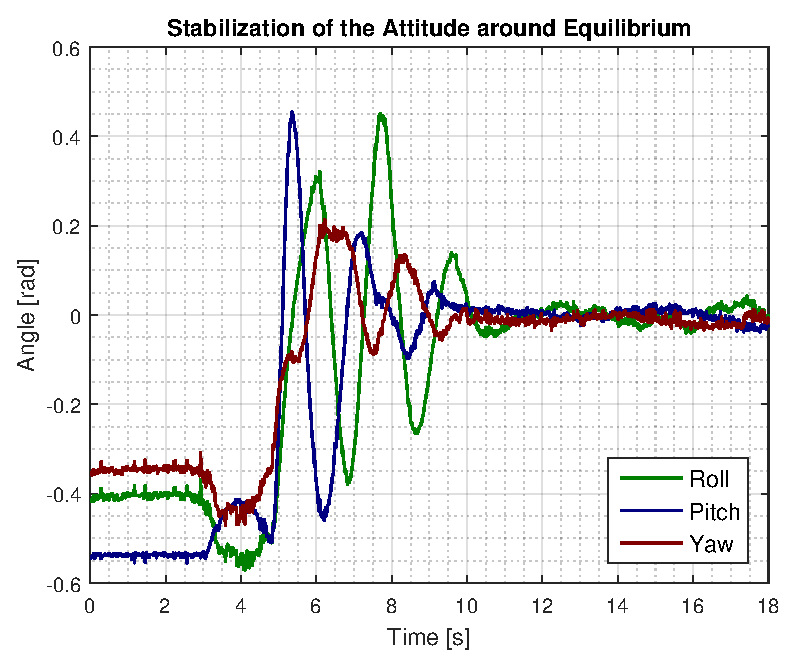
\includegraphics[scale=.7]{figures/attitudeAccept.pdf}
	\centering			
	\captionof{figure}{Testing the quadcopters ability to stabilize around equilibrium.} 
	\label{fig:attitudeAccept}
\end{figure} 
%
The three angles start with an initial condition of \SI{-0.2}{rad} for roll, \SI{-0.2}{rad} for pitch and \SI{-0.2}{rad} for yaw. After approximately five seconds, all the references are set to zero. It can be seen that the angles converge to zero in less than \SI{2}{s} for roll and pitch and approximately \SI{7}{s} for yaw. From the figure it can be seen that oscillations of approximately \SI{0.04}{rad} occur   when the attitude controller has a reference of \SI{0}{rad}. These oscillations may come from the deviations between the model and real system behavior, as the utilized parameters for the model could be different from the real system. Furthermore, certain aspects of the behavior of the quadcopter have not been taken into account.

The resolution of the measured data has been decreased to 0.01 rad to reduce the packet size, which results in a reduced delay, but can be bla bla.

In \autoref{fig:AccepttestRefTrackRoll} a reference of \SI{0.4}{rad} in roll is given to the attitude controller at approximately \SI{10}{s}.
\begin{minipage}{\linewidth}
    \begin{minipage}{0.46\linewidth}
        \begin{figure}[H]
            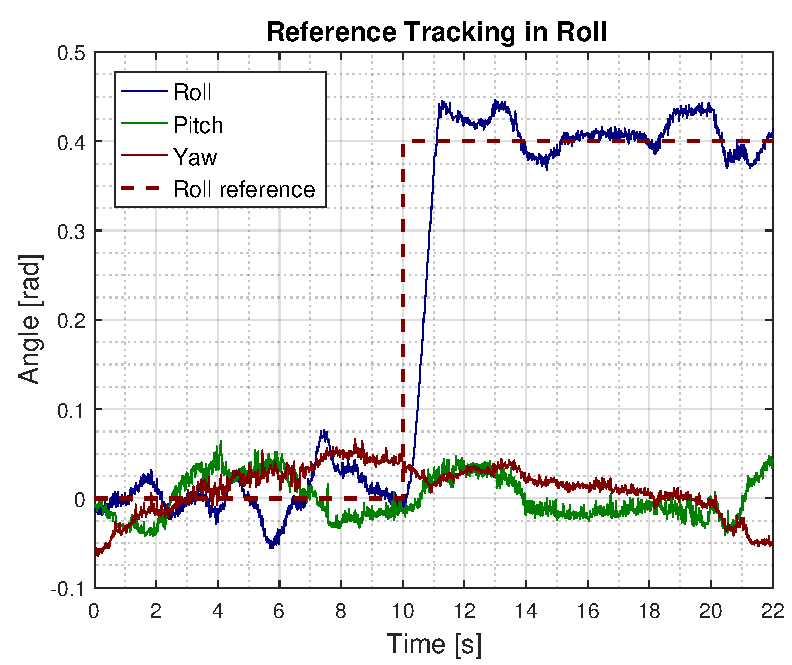
\includegraphics[scale=.55]{figures/AccepttestRefTrackRoll.pdf}
            \centering			
            \captionof{figure}{Attitude controller when tracking a roll angle reference of \SI{0.4}{rad}.}
            \label{fig:AccepttestRefTrackRoll}
        \end{figure}
    \end{minipage}
    \hspace{0.03\linewidth}
    \begin{minipage}{0.46\linewidth}
        \begin{figure}[H]
            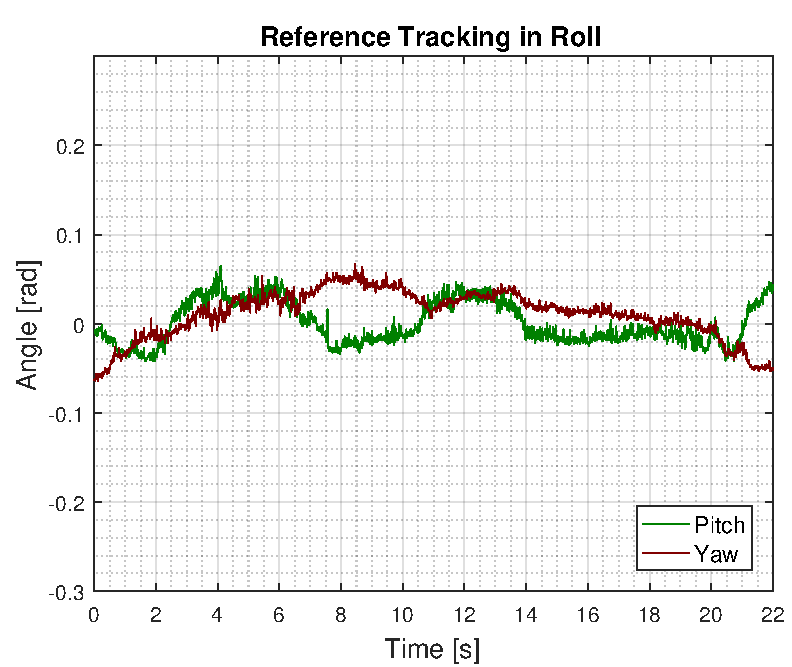
\includegraphics[scale=.55]{figures/AccepttestRefTrackRollPitchYaw.pdf}
            \centering
            \captionof{figure}{Pitch and yaw angles when a reference of \SI{0.4}{rad} in roll is given to the attitude controller.}
            \label{fig:AccepttestRefTrackRollPitchYaw}
        \end{figure}
    \end{minipage}
\end{minipage}
%
From the figure, it can be seen that it is possible for the roll to track a change in reference. This is achievable while the pitch and yaw angles remain at zero. The oscillations seen around the reference are approximately \SI{0.04}{rad}.
%
\begin{minipage}{\linewidth}
    \begin{minipage}{0.46\linewidth}
        \begin{figure}[H]
            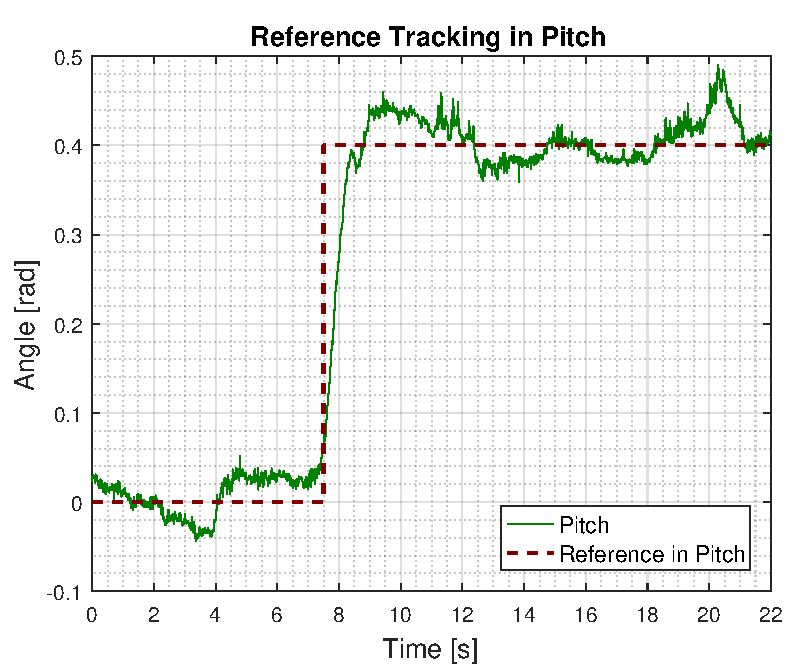
\includegraphics[scale=.55]{figures/AccepttestRefTrackPitch.pdf}
            \centering			
            \captionof{figure}{.}
            \label{fig:AccepttestRefTrackPitch}
        \end{figure}
    \end{minipage}
    \hspace{0.03\linewidth}
    \begin{minipage}{0.46\linewidth}
        \begin{figure}[H]
            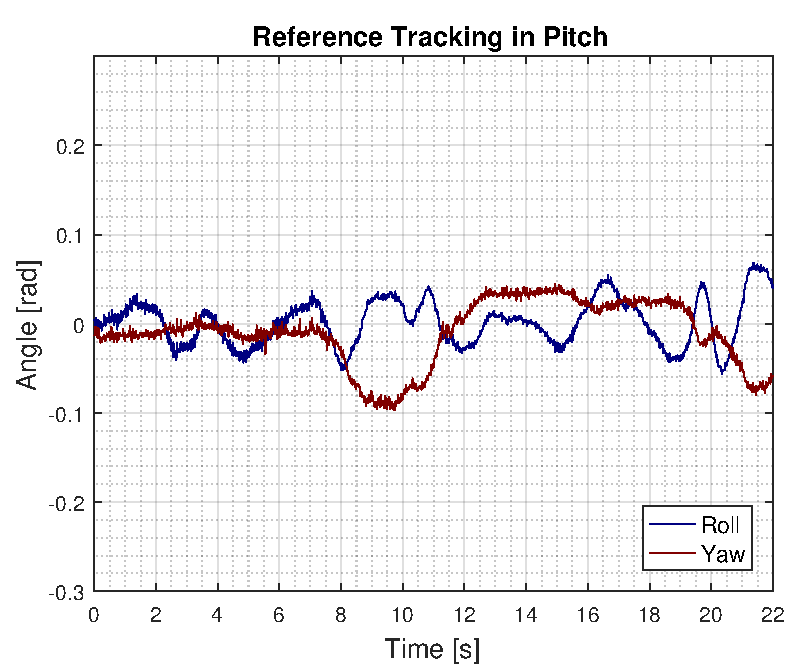
\includegraphics[scale=.55]{figures/AccepttestRefTrackPitchRollYaw.pdf}
            \centering
            \captionof{figure}{.}
            \label{fig:AccepttestRefTrackPitchRollYaw}
        \end{figure}
    \end{minipage}
\end{minipage}


\newpage

\section{Control the position in the z axis}
\textbf{Requirement:}
\textit{It shall be possible to make the quadcopter control its position in the z axis.}

\textbf{Results:}
Experimental tests reveal a non functional $z_{\mathrm{I}}$ controller implementation. However, it is believed that the designed is valid as it has been verified in simulations as depicted in \autoref{sec:TranslationalController}. As the implementation of the attitude controller functions in experimental tests, seen in \autoref{sec:accepttestAttitude}, it can be suggested that a simulated controller design could be implemented on the quadcopter and work if more time was given.


% works as well, it is a matter of time to solve the implementation issues. 



\newpage

\section{Control the position in the x and y axis}
\textbf{Requirement:}
\textit{It shall be possible to control the quadcopter in the x and y axis}

\textbf{Results:}
Experimental tests reveal a non functional $x_{\mathrm{I}}$ and $y_{\mathrm{I}}$ controller implementation. However, it is believed that the designed is valid as it has been verified in simulations as depicted in \autoref{sec:TranslationalController}. As the implementation of the attitude controller functions in experimental tests, seen in \autoref{sec:accepttestAttitude}, it can be suggested that a simulated controller design could be implemented on the quadcopter and work if more time was given.


\newpage
\section{Summary of Results}
The results of the tests are summed up in \autoref{tab:acceptance_test_results}.
\begin{table}[H] \centering
\begin{tabular}{|c|p{11cm}|c|}
\hline 
\textbf{Req. nr.} & \textbf{Requirement} & \textbf{Result} \\ 
\hline 
1 & The quadcopter should be able to receive its own position and attitude from the Vicon system each control loop, through a computer at the ground station. & \ding{51}\\ 
\hline
2 & It shall be possible to control the quadcopter's attitude. & \ding{51} \\ 
\hline 
3 & It shall be possible to make the quadcopter control its position in the z axis. & \ding{51} \\ 
\hline 
4 & It shall be possible to control the quadcopter in the x and y axis. & \ding{51} \\ 
\hline  
\end{tabular} 
\caption{Summary of acceptance test results.}
\label{tab:acceptance_test_results}
\end{table}

As can be seen, the prototype fulfils 4/4 of the set requirements. 


